\section{Laboratory Lecture 3: Stepper Motor Controller}

\subsection{Introduction}

The aim of this practice is to go over the basics of how to control a stepper motor. A stepper motor is a brushless DC electric motor that divides a full rotation in several small increments or \textit{steps}. By providing power to its coils in a specific way, we can control the position of the shaft.\medskip

Stepper motors can be unipolar or bipolar. Unipolar Stepper motors are very similar to Bipolar Stepper Motors, but are manufactured with a central tap that connects back to the power source, essentially splitting each coil into two smaller coils that can be powered independently. If required, the central tap can also be left disconnected, allowing the Unipolar Stepper Motor to be converted into a Bipolar configuration.\medskip

Bipolar Stepper Motors do not feature a central tap for dividing their solenoid coils. This makes their internal wiring slightly less complex than that of a Unipolar Motor.

\vspace{0.3cm}

\begin{figure}[H]
    \centering
    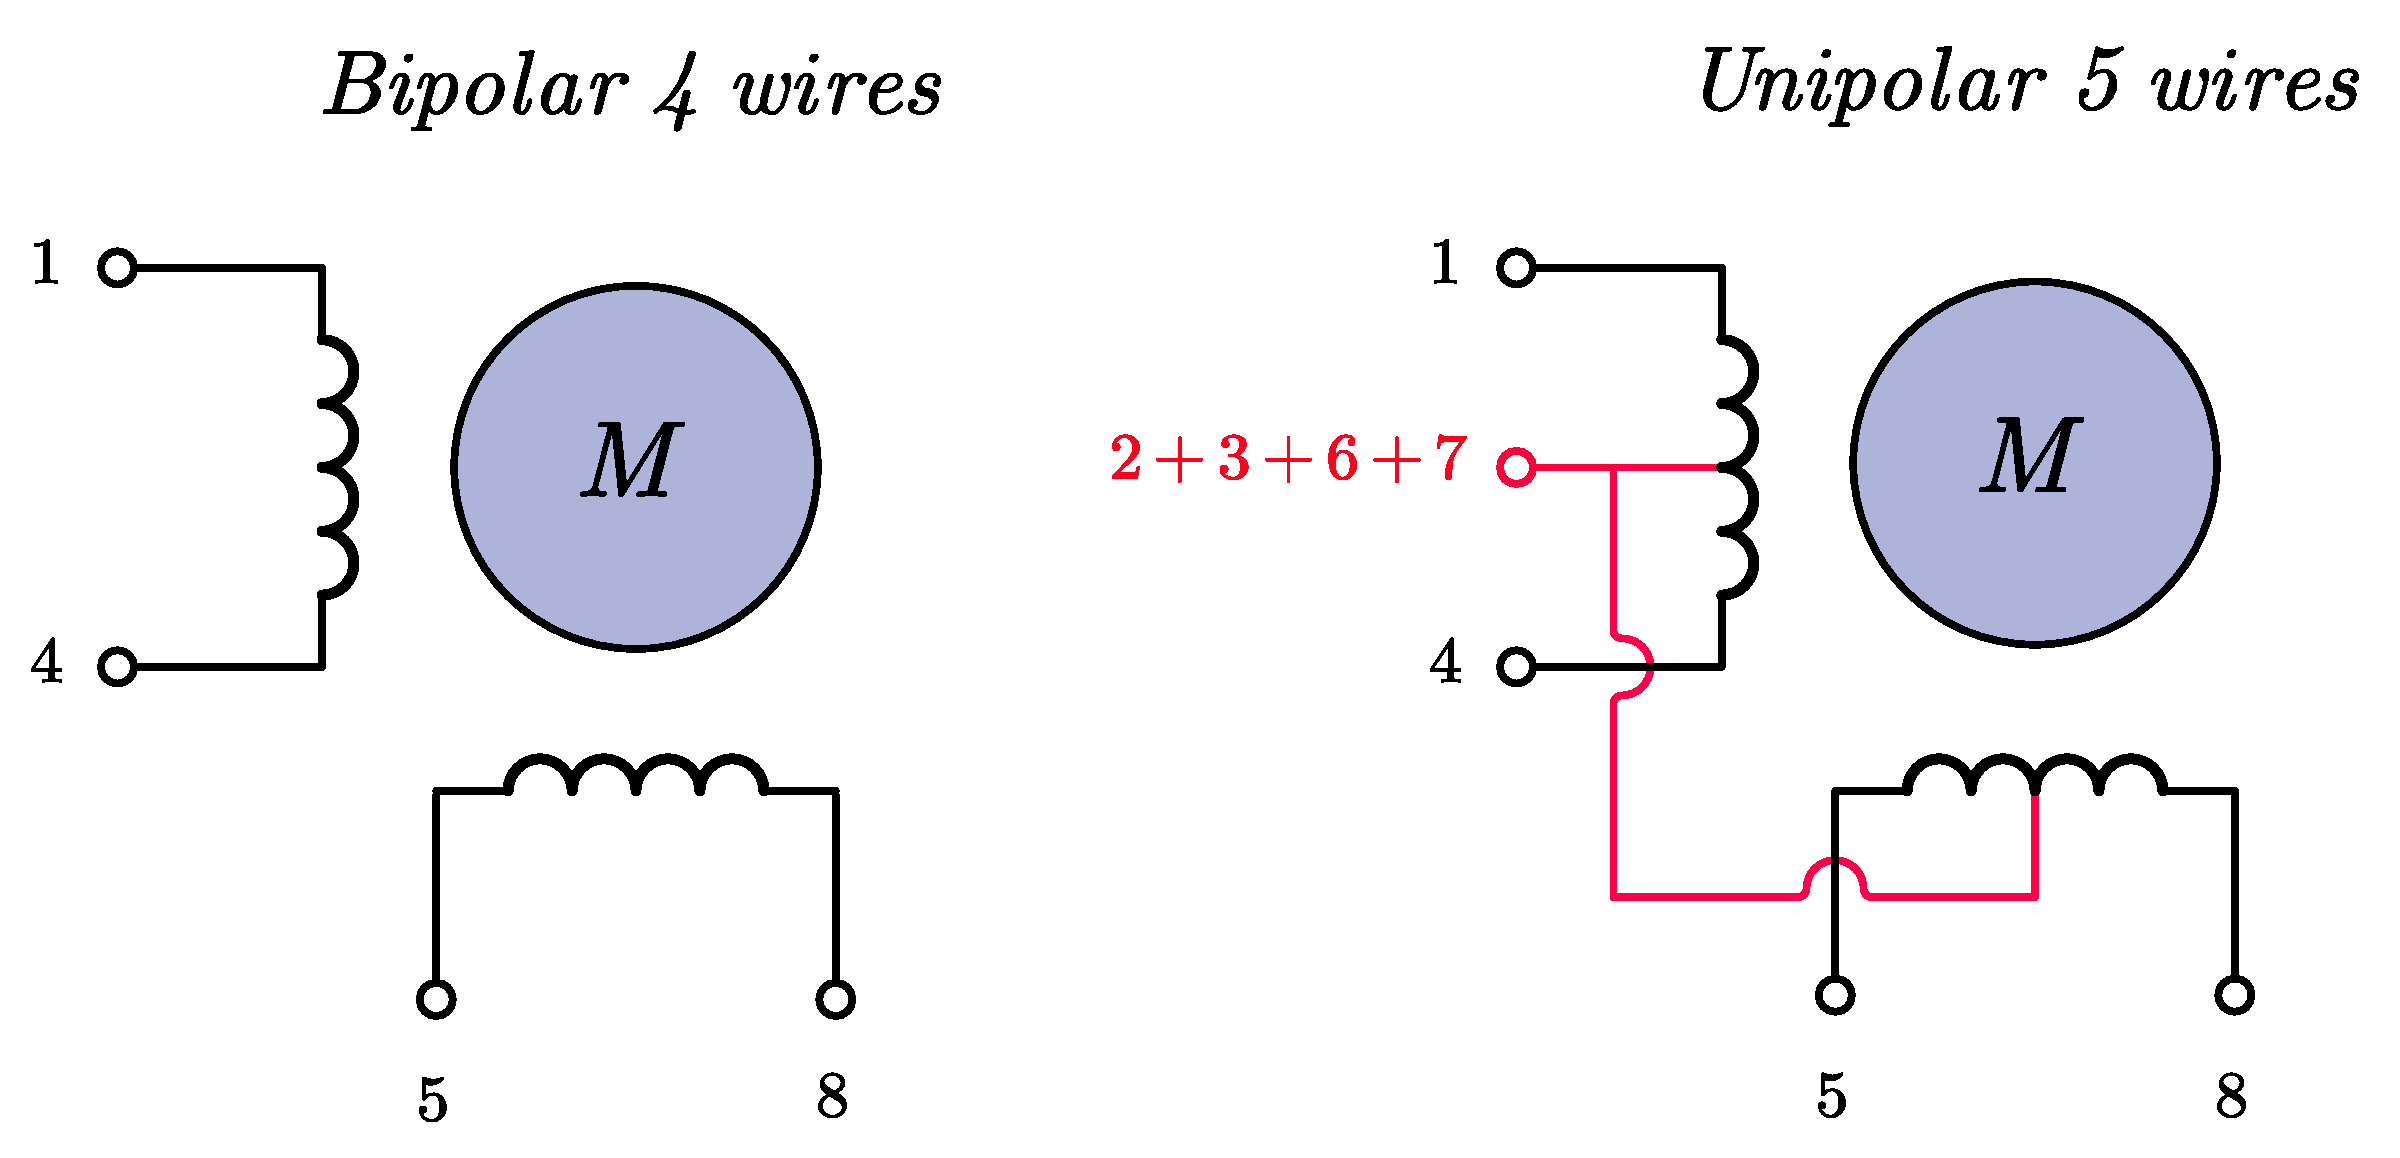
\includegraphics[scale = 0.24]{Graphics/Practice 3/GRAPHICS/STEPPER_TYPES.pdf}
    \caption{Bipolar vs. Unipolar configurations.}
    \label{fig:STEPPER_TYPE}
\end{figure}

\clearpage

\subsection{Stepper Motor Controller}

In this practice we will use the Bipolar type, in particular a NEMA 17 motor. To control it we will use a special driver, the L293D, which is basically an array or darlington transistors, in half-H configuration,  whose main objective is to take care of switching the high currents that the motors require. 

\vspace{0.3cm}

\begin{figure}[H]
    \centering
    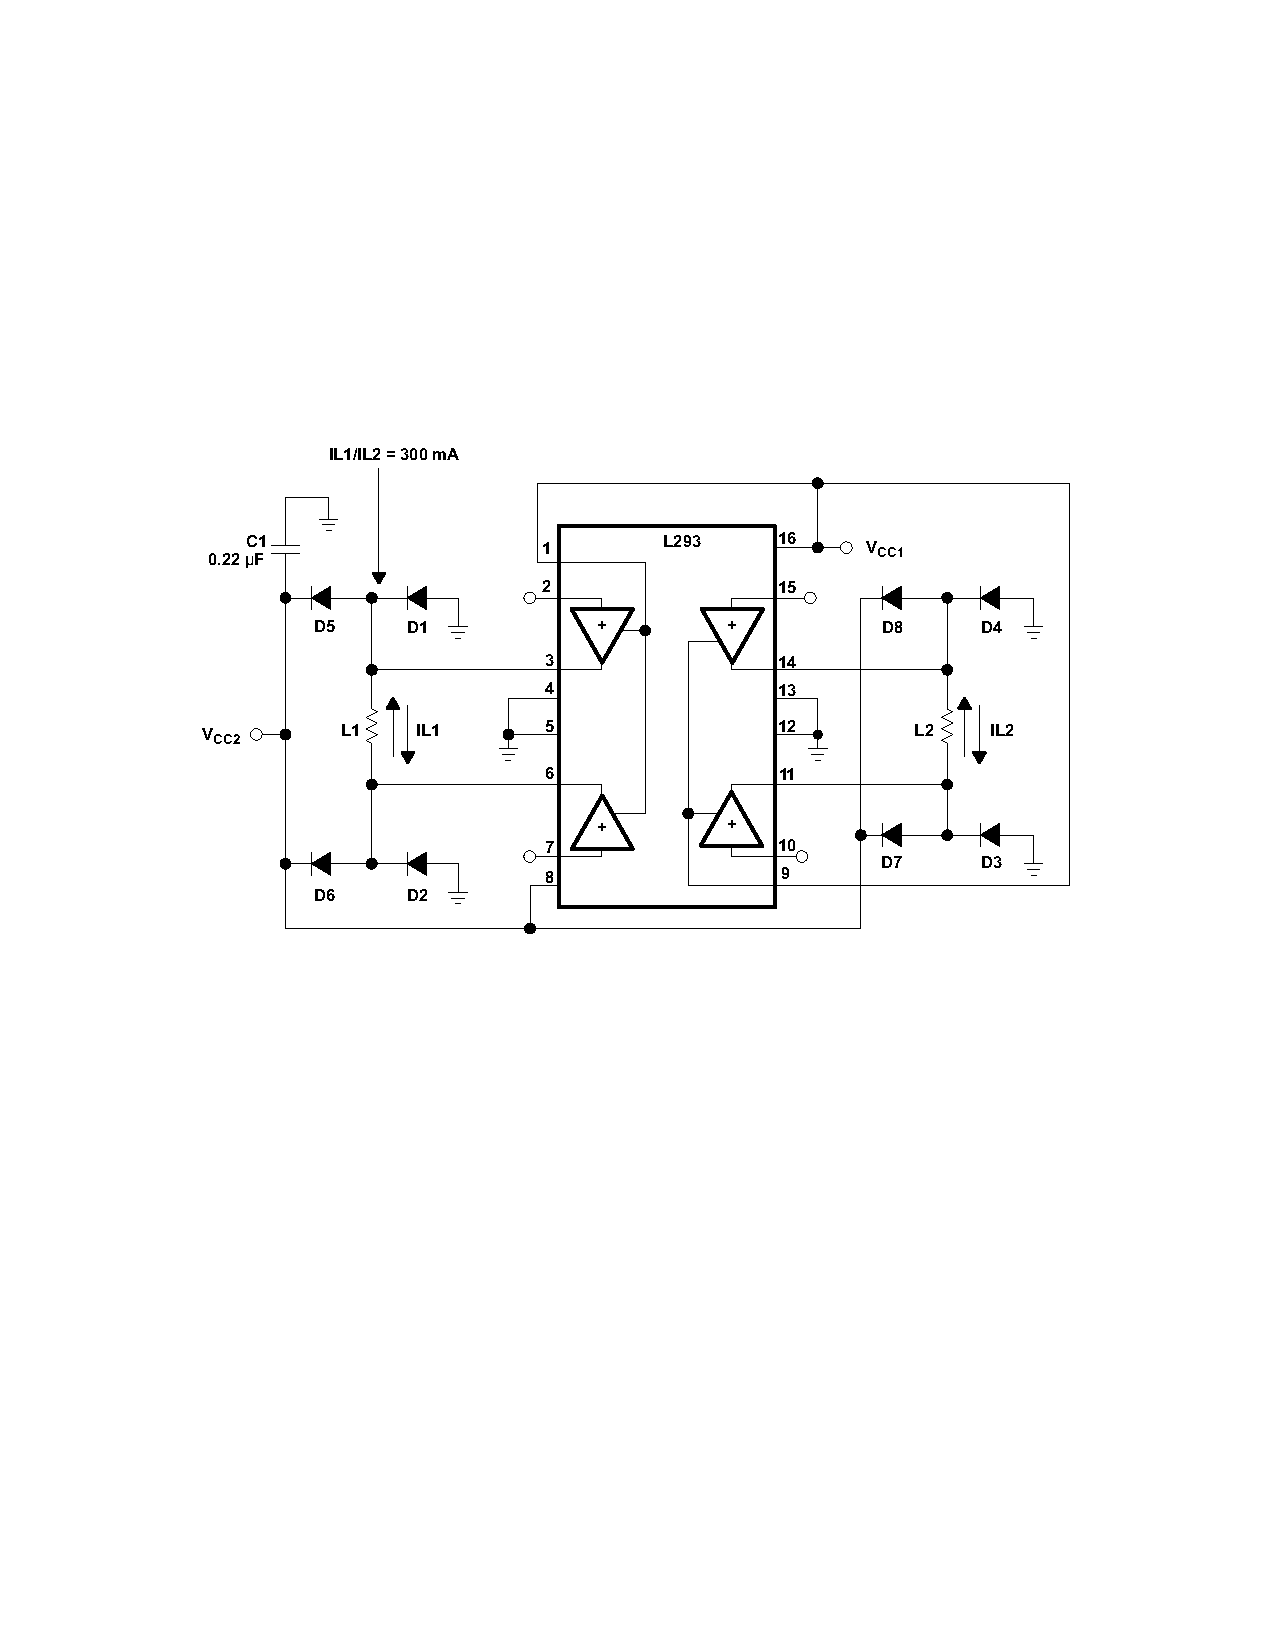
\includegraphics[scale = 0.85]{Graphics/Practice 3/GRAPHICS/DATASHEETS/L293D_INTERNAL.pdf}
    \caption{L293D Bipolar Stepper Controller. ~\autocite{L293D}}
    \label{fig:L293D}
\end{figure}

To control said driver, we will make us of the SPLD that we have been using since the beginning, the GAL22V10C and some basic VHDL code. In order to make the shaft spin in a controlled manner, we have to take into account the phase current waveforms, i.e. the pulses that we have to send to the driver to cause a step change and the order in which they must be sent. This information can be seen below:

\vspace{0.3cm}

\begin{table}[ht]
    \centering
        \begin{tabular}[t]{lcccc}
            \toprule
            &\textbf{Step}&\textbf{Full-Step [1.8\textdegree]}&\textbf{Wave-Step [1.8\textdegree]}&\textbf{Half-Step [0.9\textdegree]}\\
            \midrule
            & 0 & 1010 & 1000 & 1010\\
            & 1 & 1001 & 0001 & 1000\\
            & 2 & 0101 & 0100 & 1001\\
            & 3 & 0110 & 0010 & 0001\\
            & 4 &      &      & 0101\\
            & 5 &      &      & 0100\\
            & 6 &      &      & 0110\\
            & 7 &      &      & 0010\\
            \bottomrule
        \end{tabular}
        \caption{Phase Current Waveforms. ~\autocite{SLIDES_3}}
        \label{table: PHASE_CURRENT_WAVEFORMS}
\end{table}

\subsubsection{VHDL Code}

As we have seen in Table \ref{table: PHASE_CURRENT_WAVEFORMS}, there are 3 different ways in which we can control the rotation of the stepper motor, namely, full-step, wave-step and half-step. Each of them present advantages and disadvantages. For instance, \textit{Half-Steps} can deliver a higher precision, since every step only spins the shaft 0.9\textdegree as opposed to \textit{full-step} and \textit{wave-step}, which spin it 1.8\textdegree. This increase in performance reduces the output torque significantly, so there is a clear trade-off between both variables that one must consider. In addition to this, \textit{Wave-step} mode is more visually appealing, as the transitions between states are not as choppy as with the other ones.\medskip

Due to the limitations that the GAL22V10C possesses, it is not possible to fit the 3 control modes in the same SPLD. That's why we have developed 3 different codes, one for each, that can be seen below:

\paragraph{Full Step}
\label{sec:FULL_STEP}

\begin{code}{vhdl}
library ieee;
use ieee.std_logic_1164.all;

entity STEPPER_FS is
  port(CLK: in std_logic;
       DIR: in std_logic;
       MOTOR: out std_logic_vector(3 downto 0)
       );
end STEPPER_FS;

architecture ARCH of STEPPER_FS is
  begin
    process(CLK)
      variable COUNT: std_logic_vector(3 downto 0);
        begin
          if(CLK'EVENT and CLK='1') then

            if(DIR='0') then
              case COUNT is
                when "0000" => COUNT := "1010";
                when "1010" => COUNT := "1001";
                when "1001" => COUNT := "0101";
                when "0101" => COUNT := "0110";
                when "0110" => COUNT := "1010";
                when others => COUNT := "0000";
              end case;
              
              
              
                else
                  case COUNT is
                    when "0000" => COUNT := "0110";
                    when "0110" => COUNT := "0101";
                    when "0101" => COUNT := "1001";
                    when "1001" => COUNT := "1010";
                    when "1010" => COUNT := "0110";
                    when others => COUNT := "0000";
                  end case;
            end if;
          end if;
        
          MOTOR <= COUNT;
          
    end process;
end ARCH;
\end{code}

As we have previously mentioned, \textit{Full Step} phase control provides the highest torque of all, though the transitions tend to look quite choppy. This mode and the \textit{Wave Step} one provide a maximum accuracy of 1.8\textdegree \, per step, which means that a full 360\textdegree \, rotation would require 200 steps.\medskip

The code that we have included moves the shaft one step (forwards or backwards) whenever a \textit{PGT} occurs. This indicates that the process is synchronous. Besides, we can also find a direction pin which changes the direction of the spin when a positive signal is applied to it.

\paragraph{Wave Step}

\begin{code}{vhdl}
library ieee;
use ieee.std_logic_1164.all;

entity STEPPER_WS is
  port(CLK: in std_logic;
       DIR: in std_logic;
       MOTOR: out std_logic_vector(3 downto 0)
       );
end STEPPER_WS;

architecture ARCH of STEPPER_WS is
  begin
    process(CLK)
      variable COUNT: std_logic_vector(3 downto 0);
        begin
          if(CLK'EVENT and CLK='1') then

            if(DIR='0') then
              case COUNT is
                when "0000" => COUNT := "1000";
                when "1000" => COUNT := "0001";
                when "0001" => COUNT := "0100";
                when "0100" => COUNT := "0010";
                when "0010" => COUNT := "1000";
                when others => COUNT := "0000";
              end case;
              
                else
                  case COUNT is
                    when "0000" => COUNT := "0010";
                    when "0010" => COUNT := "0100";
                    when "0100" => COUNT := "0001";
                    when "0001" => COUNT := "1000";
                    when "1000" => COUNT := "0010";
                    when others => COUNT := "0000";
                  end case;
            end if;
          end if;
        
          MOTOR <= COUNT;
          
    end process;
end ARCH;
\end{code}

This code describes the \textit{Wave Step} phase control sequence. Wave Stepping is usually used when the smoothness of the output rotation is important. As per the last mode, this mode has a high torque but its trade-off is a reduction in its accuracy. \medskip

The rest of the code remains the same as the last one.

\paragraph{Half Step}

\begin{code}{vhdl}
library ieee;
use ieee.std_logic_1164.all;

entity STEPPER_HS is
  port(CLK: in std_logic;
       DIR: in std_logic;
       MOTOR: out std_logic_vector(3 downto 0)
       );
end STEPPER_HS;

architecture ARCH of STEPPER_HS is
  begin
    process(CLK)
      variable COUNT: std_logic_vector(3 downto 0);
        begin
          if(CLK'EVENT and CLK='1') then

            if(DIR='0') then
              case COUNT is
                when "0000" => COUNT := "1010";
                when "1010" => COUNT := "1000";
                when "1000" => COUNT := "1001";
                when "1001" => COUNT := "0001";
                when "0001" => COUNT := "0101";
                when "0101" => COUNT := "0100";
                when "0100" => COUNT := "0110";
                when "0110" => COUNT := "0010";
                when "0010" => COUNT := "1010";
                when others => COUNT := "0000";                            
            end case;
              
                else
                  case COUNT is
                    when "0000" => COUNT := "0010";
                    when "0010" => COUNT := "0110";
                    when "0110" => COUNT := "0100";
                    when "0100" => COUNT := "0101";
                    when "0101" => COUNT := "0001";
                    when "0001" => COUNT := "1001";
                    when "1001" => COUNT := "1000";
                    when "1000" => COUNT := "1010";
                    when "1010" => COUNT := "0010";
                    when others => COUNT := "0000";
                  end case;
            end if;
          end if;
        
          MOTOR <= COUNT;
          
    end process;
end ARCH;
\end{code}

In addition, we can find the \textit{Half Step} phase control sequence. As we can see, this code is longer than the last 2 codes. This is due to the fact that it has some intermediate states which help smooth out the rotation by getting rid of most of the chopping that characterizes the latter.


\subsubsection{Proteus Simulation and Assembly}

After discussing the code, we will move on to the simulation of the circuit. For this we will use ISIS Proteus once again. Even though Figure \ref{fig:L293D} may look cumbersome, in actuality, we only have to connect the 2 coils to the driver's output and the 4 direction pins to its inputs following this fashion:\medskip

\begin{figure}[H]
    \centering
    
    \ifnum\value{ANIMATION}=1 {
        \animategraphics[controls,loop,scale=0.8]{1}{Graphics/Practice 3/GRAPHICS/ANIMATION/F}{0}{8}
    } 
    \else {
        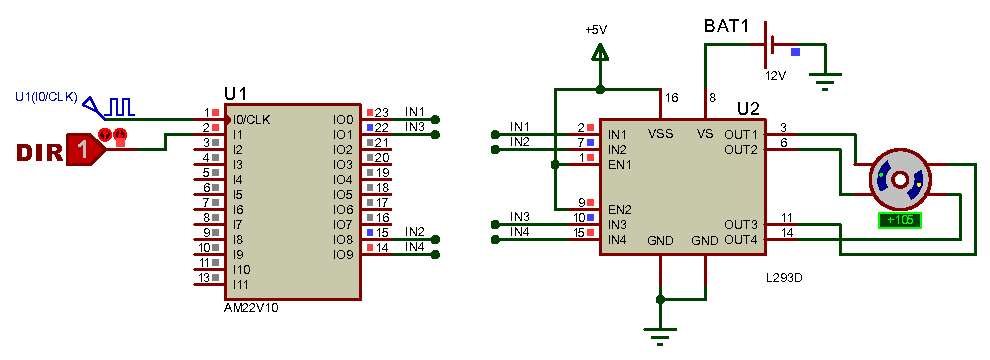
\includegraphics[scale=0.8]{Graphics/Practice 3/GRAPHICS/ANIMATION/F5.PDF}
    }\fi
    
    \caption{Stepper with rotation direction control.}
    \label{fig:STEPPER_ROTATION}
\end{figure}

The I/O pins that we used are the ones that the the compiler assigned by default. They are displayed in the Chip Report (Figure \ref{fig:CHIP_REPORT}).\medskip

Assembling the circuit is just a matter of manually connecting everything following the schematic of Figure \ref{fig:STEPPER_ROTATION}. To provide a clock signal we have used a signal generator which output has been set to a TTL level, 0 to 5V, and its frequency to 1 Hz.  

\clearpage